\documentclass{beamer}
\usepackage{lesson}
\usepackage{amsmath}
% \setbeamertemplate{footline}[frame number]

\title{From Newton's Laws to Modelling Black Holes}
\subtitle{The Power of Numerical Methods}
\author{Wenkang Xin}

\begin{document}

\frame{\titlepage}


\begin{frame}{Introduction}
    \begin{center}
        {\Large What is the \textbf{greatest} achievement of science?}

        \vspace{3cm}

        Quantum mechanics? General relativity? The standard model?
    \end{center}
\end{frame}


\begin{frame}{Introduction}
    \begin{center}
        {\Large What is the \textbf{greatest} achievement of science?}

        \vspace{3cm}

        \textbf{Ability to predict the future,}

        \vspace{0.5cm}

        using, for example, Newton's laws.
    \end{center}
\end{frame}


\begin{frame}{Contents}
    \tableofcontents
\end{frame}


\section{Newton's Laws}


\begin{frame}{Newton's Laws}
    \begin{center}
        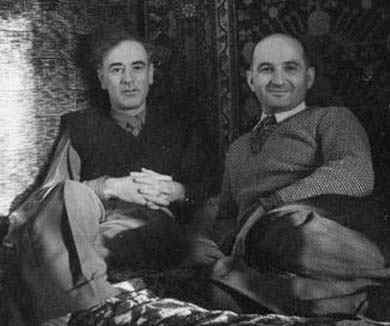
\includegraphics[width=0.5\textwidth]{asset/landau_lifshitz.jpeg}
    \end{center}

    \begin{quote}
        If all the co-ordinates and velocities (of a system) are simultaneously specified, it is known from experience that the state of the system is completely determined and that its subsequent motion can, \textbf{in principle}, be calculated.
    \end{quote}

    \footnotetext{L.D. Landau and E.M. Lifshitz.}
\end{frame}


\begin{frame}{Newton's Laws}
    \textbf{In principle}, we can predict the future using Newton's second law:

    \vspace{0.5cm}

    \begin{equation}
        \mathbf{F} = m \mathbf{a} = m \frac{\mathrm{d}^{2} \mathbf{r}}{\mathrm{d}t^{2}}
    \end{equation}

    \vspace{0.5cm}

    Once we know the force, we can solve the differential equation.
\end{frame}


\begin{frame}{Newton's Laws}
    Imagine you are a rocket moving in space towards Mother Earth. Your dynamics is a constant updating of the state vector:

    \vspace{0.5cm}

    \begin{equation}
        \begin{pmatrix}
            x \\
            v
        \end{pmatrix}
        \xrightarrow{\delta t}
        \begin{pmatrix}
            x + v \delta t \\
            v + a \delta t
        \end{pmatrix}
    \end{equation}

    \vspace{0.5cm}

    How do we know the acceleration $a$?
\end{frame}


\section{Numerical Methods}


\begin{frame}{Numerical Methods}
    \begin{columns}
        \column{0.5\textwidth}
        \centering
        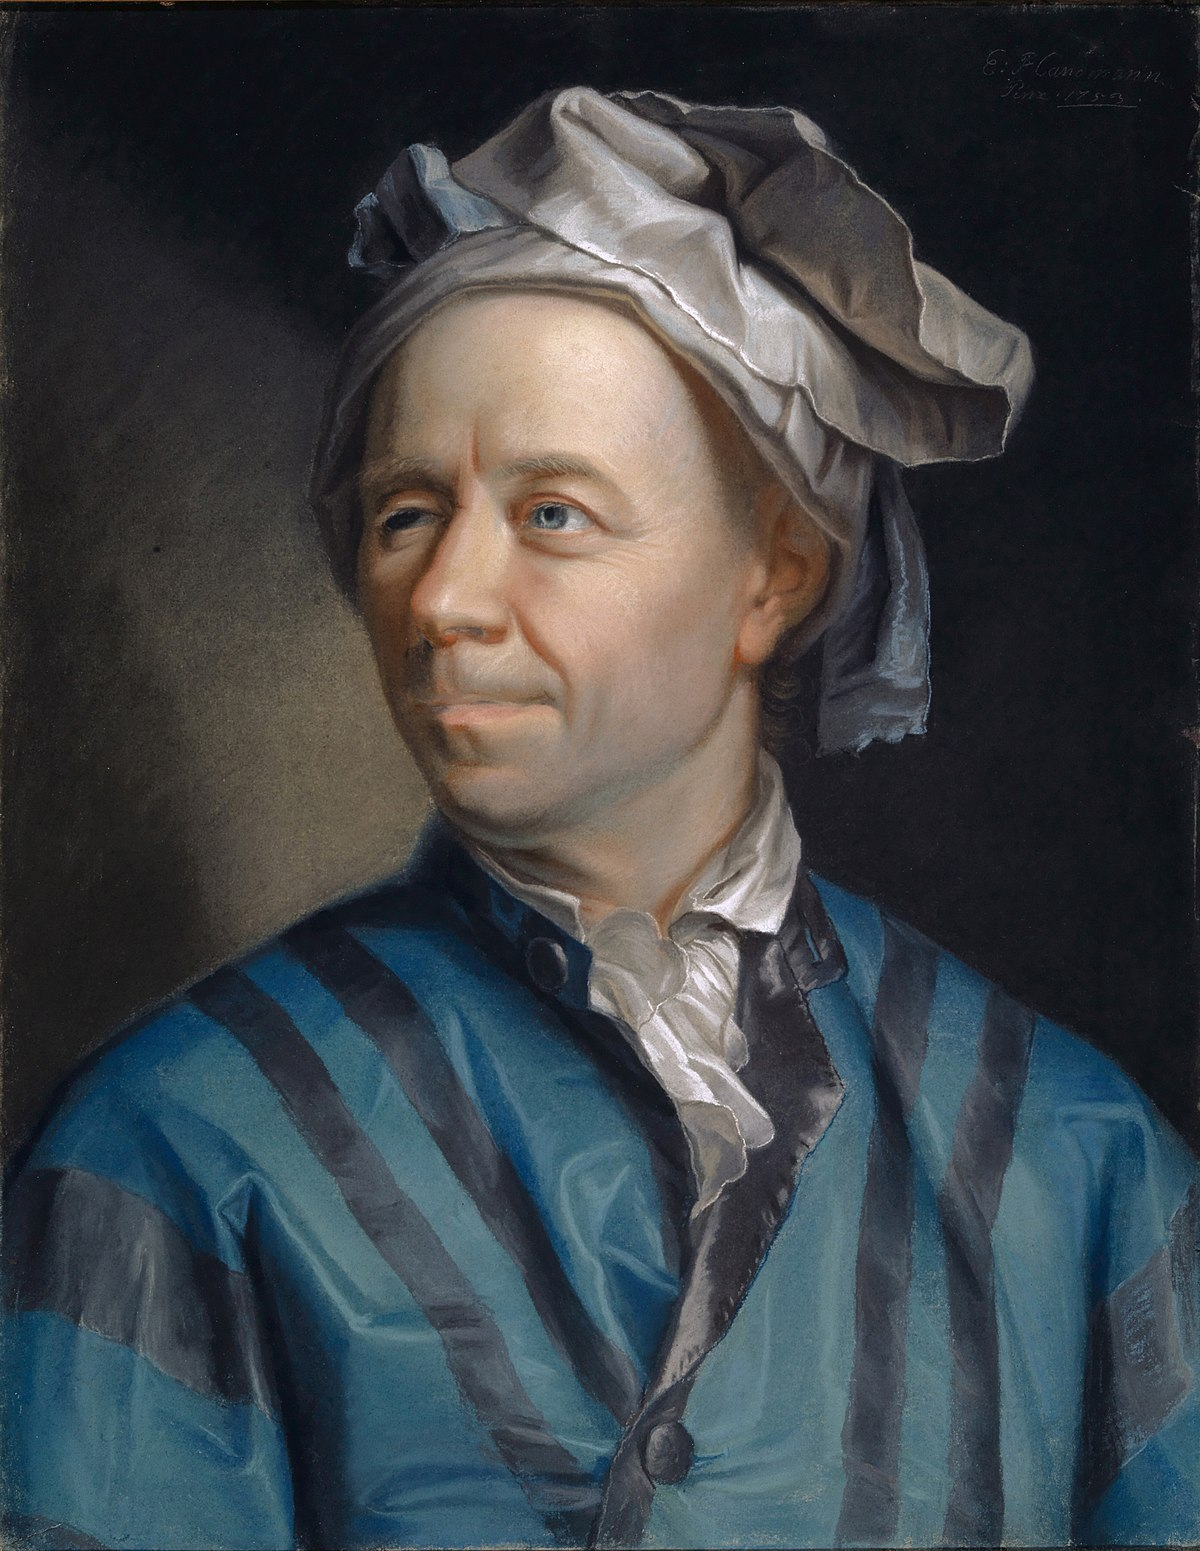
\includegraphics[width=\textwidth]{asset/euler.jpg}
        \column{0.5\textwidth}
        \centering
        What we just did is called the \textbf{Euler's method}.

        \vspace{0.5cm}

        It is a general method of solving ordinary differential equations.
    \end{columns}

    \footnotetext{Leonhard Euler (1707-1783).}
\end{frame}


\begin{frame}{Numerical Methods}
    Consider the following differential equation:

    \vspace{0.5cm}

    \begin{equation}
        \frac{\mathrm{d}y}{\mathrm{d}t} = -15y \quad y(0) = 1
    \end{equation}

    \vspace{0.5cm}

    We know the solution is:

    \vspace{0.5cm}

    \begin{equation}
        y(t) = e^{-15t}
    \end{equation}

    \vspace{0.5cm}

    Let's see how Euler's method performs with different step sizes.
\end{frame}


\begin{frame}{Numerical Methods}
    \begin{center}
        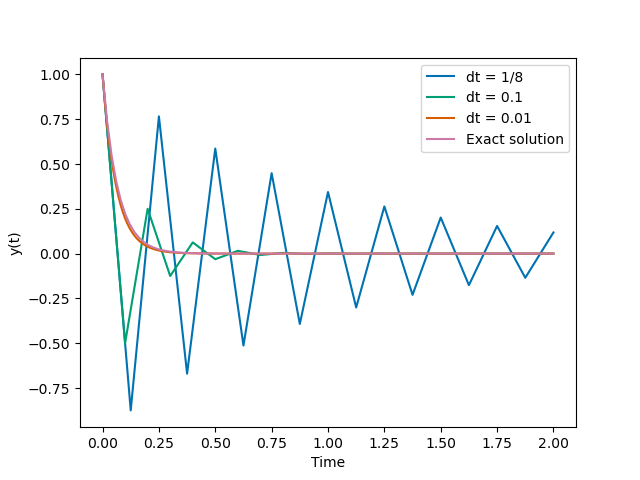
\includegraphics[width=0.95\textwidth]{asset/euler_method.png}
    \end{center}
\end{frame}


\begin{frame}{Numerical Methods}
    There are at least two problems with the naive Euler's method:

    \vspace{0.5cm}

    \begin{enumerate}
        \item It is (very) \textbf{inaccurate} for large step sizes.
        \item It becomes (very) \textbf{slow} for small step sizes.
    \end{enumerate}
\end{frame}


\begin{frame}{Numerical Methods - Go to Higher Orders}
    The Euler's method is naive in a sense that it is too `local'.

    \vspace{0.5cm}

    We could have 'scouted' ahead a bit and use the average of acceleration there and our current position.
\end{frame}


\begin{frame}{Numerical Methods - Go to Higher Orders}
    \begin{columns}
        \column{0.5\textwidth}
        \centering
        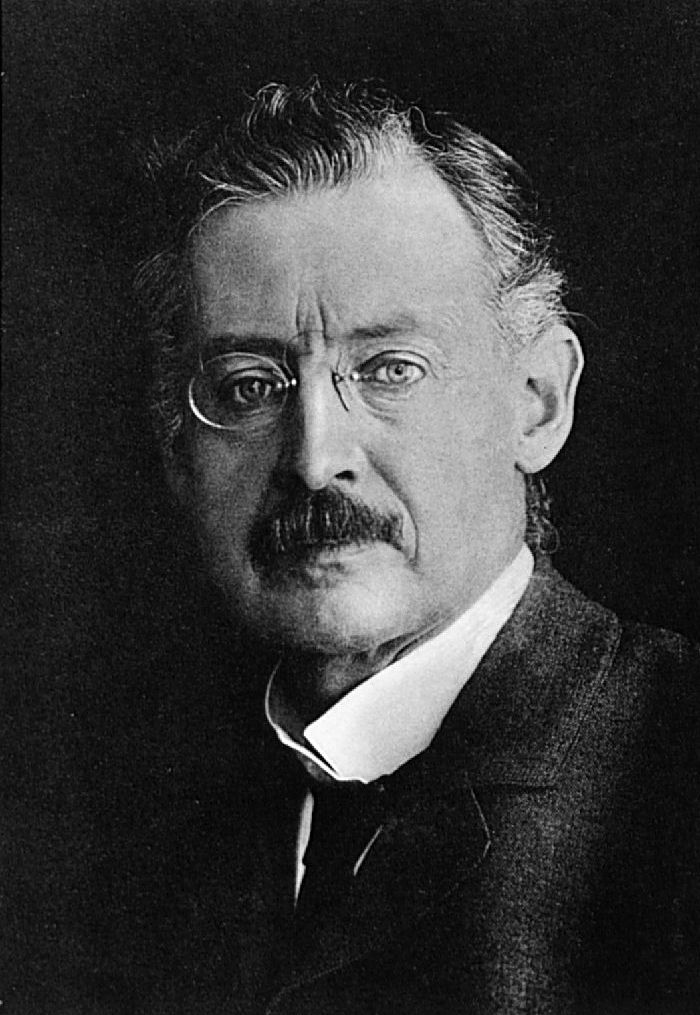
\includegraphics[width=\textwidth]{asset/runge.jpg}
        \column{0.5\textwidth}
        \centering
        Let us go as far as four steps ahead!

        \vspace{0.5cm}

        \textbf{Runge-Kutta methods} are a family of numerical methods for ODEs.

        \vspace{0.5cm}

        The most famous is the RK4 method.
    \end{columns}

    \footnotetext{Carl David Tolmé Runge (1856-1927).}
\end{frame}


\begin{frame}{Numerical Methods - Adapt Your Step}
    The Euler's method is also too 'dumb' because it only knows a \textbf{fixed step size}.

    \centering
    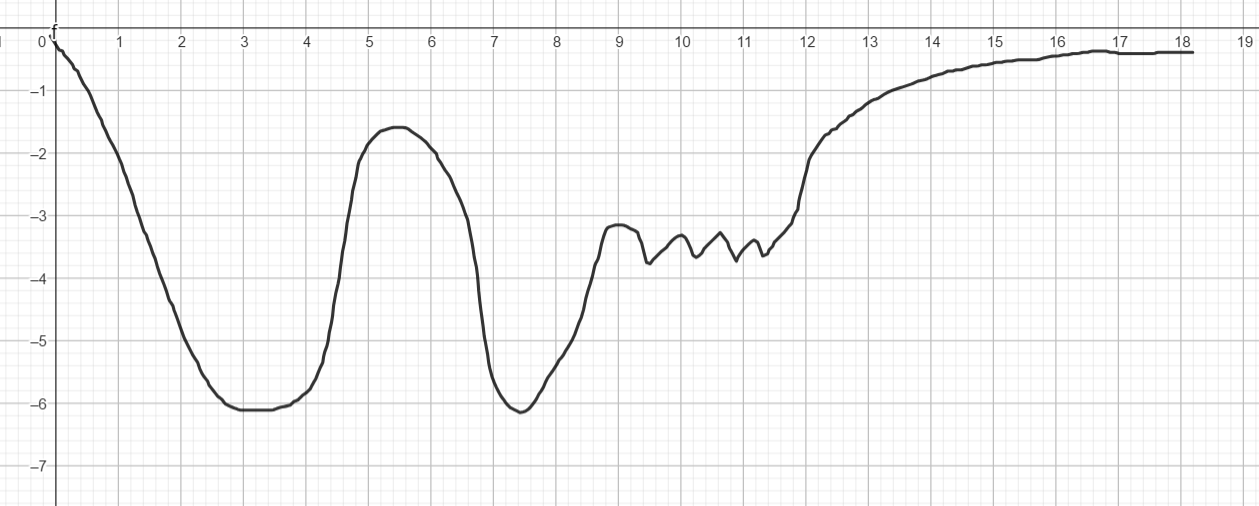
\includegraphics[width=\textwidth]{asset/func.png}
\end{frame}


\begin{frame}{Numerical Methods - Adapt Your Step}
    To know when and how to adapt the step size, we require a rough \textbf{estimate of the error}.

    \vspace{0.5cm}

    RK(F)45 method is a viable choice, which uses both 4th and 5th order results to estimate the error.
\end{frame}


\section{Foraging to Black Holes}


\begin{frame}{Foraging to Black Holes}
    Instead of a rocket, what if we are photons travelling towards a black hole?

    \vspace{0.5cm}

    \begin{center}
        {\Large What even is a black hole?}
    \end{center}
\end{frame}


\begin{frame}{Foraging to Black Holes}
    \begin{columns}
        \column{0.5\textwidth}
        \centering
        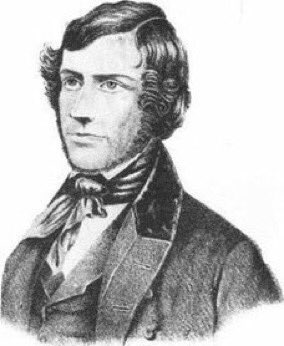
\includegraphics[width=\textwidth]{asset/michell.jpg}
        \column{0.5\textwidth}
        \centering
        \textbf{John Michell} first to proposed the existence of `black holes'.

        \vspace{0.5cm}

        Alas, he was too far ahead of his time.

        \vspace{0.5cm}

        Scientists then did not have the tools to investigate his ideas.
    \end{columns}

    \footnotetext{John Michell (1724-1793).}
\end{frame}


\begin{frame}{Foraging to Black Holes}
    \begin{columns}
        \column{0.5\textwidth}
        \centering
        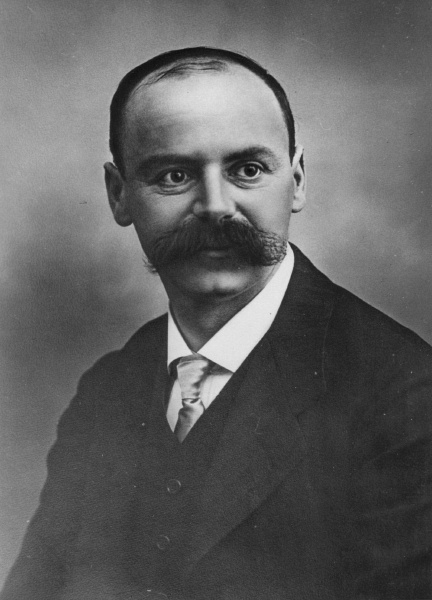
\includegraphics[width=\textwidth]{asset/schwarzschild.jpg}
        \column{0.5\textwidth}
        \centering
        \textbf{Albert Einstein} published the general theory of relativity in 1915 along with his field equations.

        \vspace{0.5cm}

        \textbf{Karl Schwarzschild} found the first solution to the equations in 1916.

        \vspace{0.5cm}

        From his solutions, the concept of a black hole emerged.
    \end{columns}

    \footnotetext{Karl Schwarzschild (1873-1916).}
\end{frame}


\begin{frame}{Foraging to Black Holes}
    It was soon realised that BHs are very simple objects with only three properties:

    \vspace{0.5cm}

    \begin{enumerate}
        \item Mass $M$
        \item Charge $Q$ (theorised to be zero)
        \item Spin $J$
    \end{enumerate}
\end{frame}


\begin{frame}{Foraging to Black Holes}
    BHs are often found in binary systems and a process called \textbf{accretion} occurs to give rise to \textbf{accretion disks}.

    \vspace{0.5cm}

    These disks get so hot ($\sim 10^{7}K$) that they emit some of the most energetic radiation in the universe.
\end{frame}


\begin{frame}{Foraging to Black Holes - Some GR}
    You have probably heard of mass 'bending' space in GR. How do we quantify this effect? Using a metric!

    \vspace{0.5cm}

    \begin{equation*}
        \begin{pmatrix} -1 & 0 & 0 & 0 \\ 0 & 1 & 0 & 0 \\ 0 & 0 & 1 & 0 \\ 0 & 0 & 0 & 1 \end{pmatrix} \to \begin{pmatrix} -\left( 1 - \frac{r_{s}}{r} \right) & 0 & 0 & 0 \\ 0 & \frac{1}{\left( 1 - \frac{r_{s}}{r} \right)} & 0 & 0 \\ 0 & 0 & r^{2} & 0 \\ 0 & 0 & 0 & r^{2}\sin^{2}{\theta} \end{pmatrix}
    \end{equation*}
\end{frame}


\begin{frame}{Foraging to Black Holes - Some GR}
    The motion of a photon is governed by the geodesic equation:

    \vspace{0.5cm}

    \begin{equation*}
        \frac{\mathrm{d}^{2}x^{\mu}}{\mathrm{d}\lambda^{2}} + \Gamma^{\mu}_{\nu\sigma}\frac{\mathrm{d}x^{\nu}}{\mathrm{d}\lambda}\frac{\mathrm{d}x^{\sigma}}{\mathrm{d}\lambda} = 0
    \end{equation*}

    \vspace{0.5cm}

    This can be numerically integrated!
\end{frame}


\section{Exciting Science}


\begin{frame}{Exciting Science - Ray Tracing}
    We can use C++ (for its speed) to \textbf{simulate} how photons from an accretion disk travel to an observer.

    \vspace{0.5cm}

    \centering
    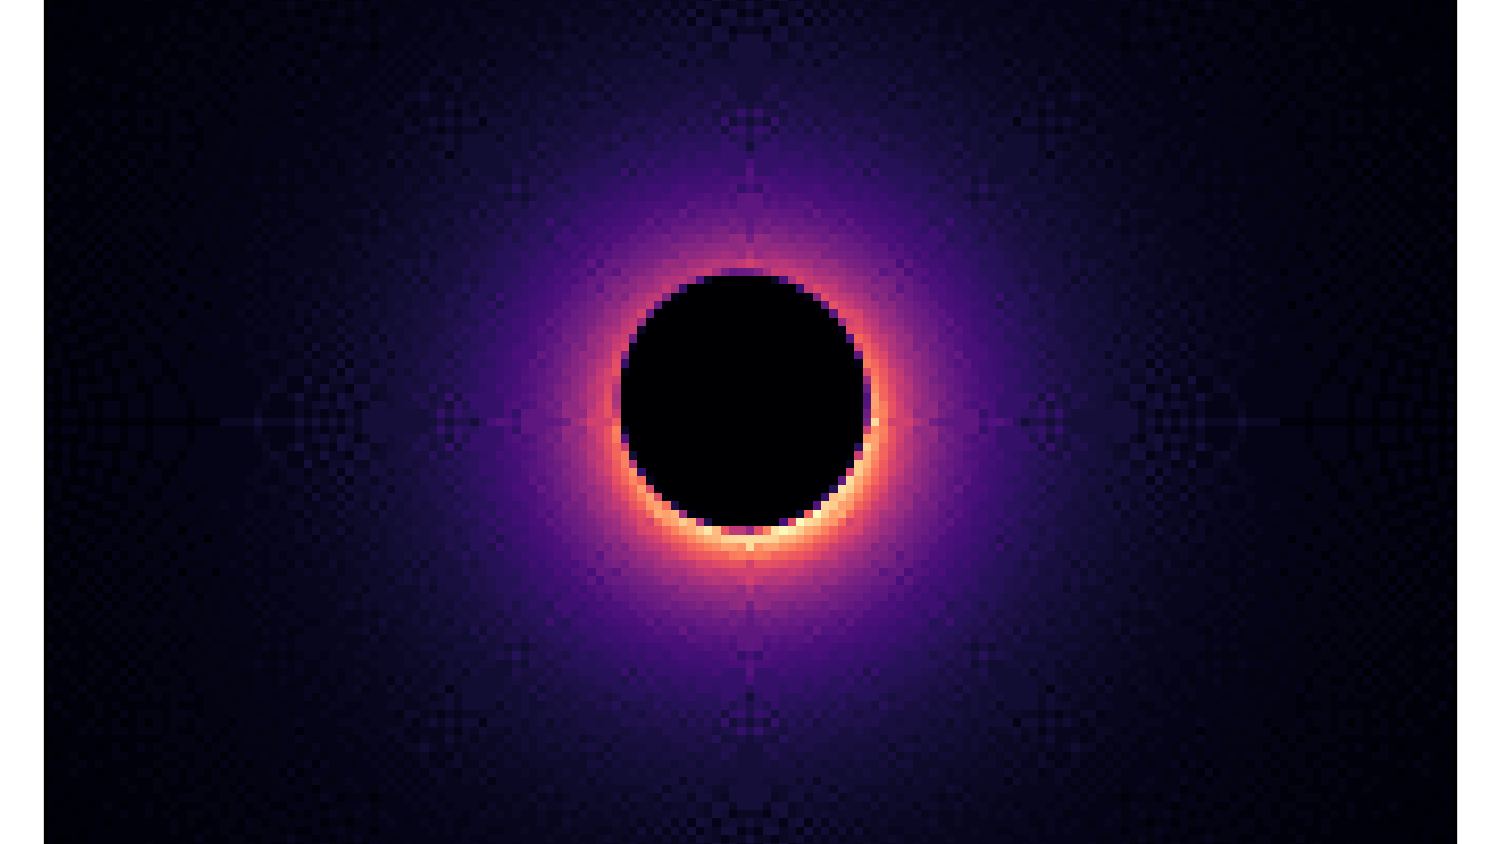
\includegraphics[width=0.90\textwidth]{asset/bh_alt.png}

    \footnotetext{spin = 0.95, inclination = 20 deg}
\end{frame}


\begin{frame}{Exciting Science - Actual Value}
    Besides simulating a BH on your PC, the algorithm also gives us a \textbf{spectrum} that contains key information about the BH.

    \vspace{0.5cm}

    \centering
    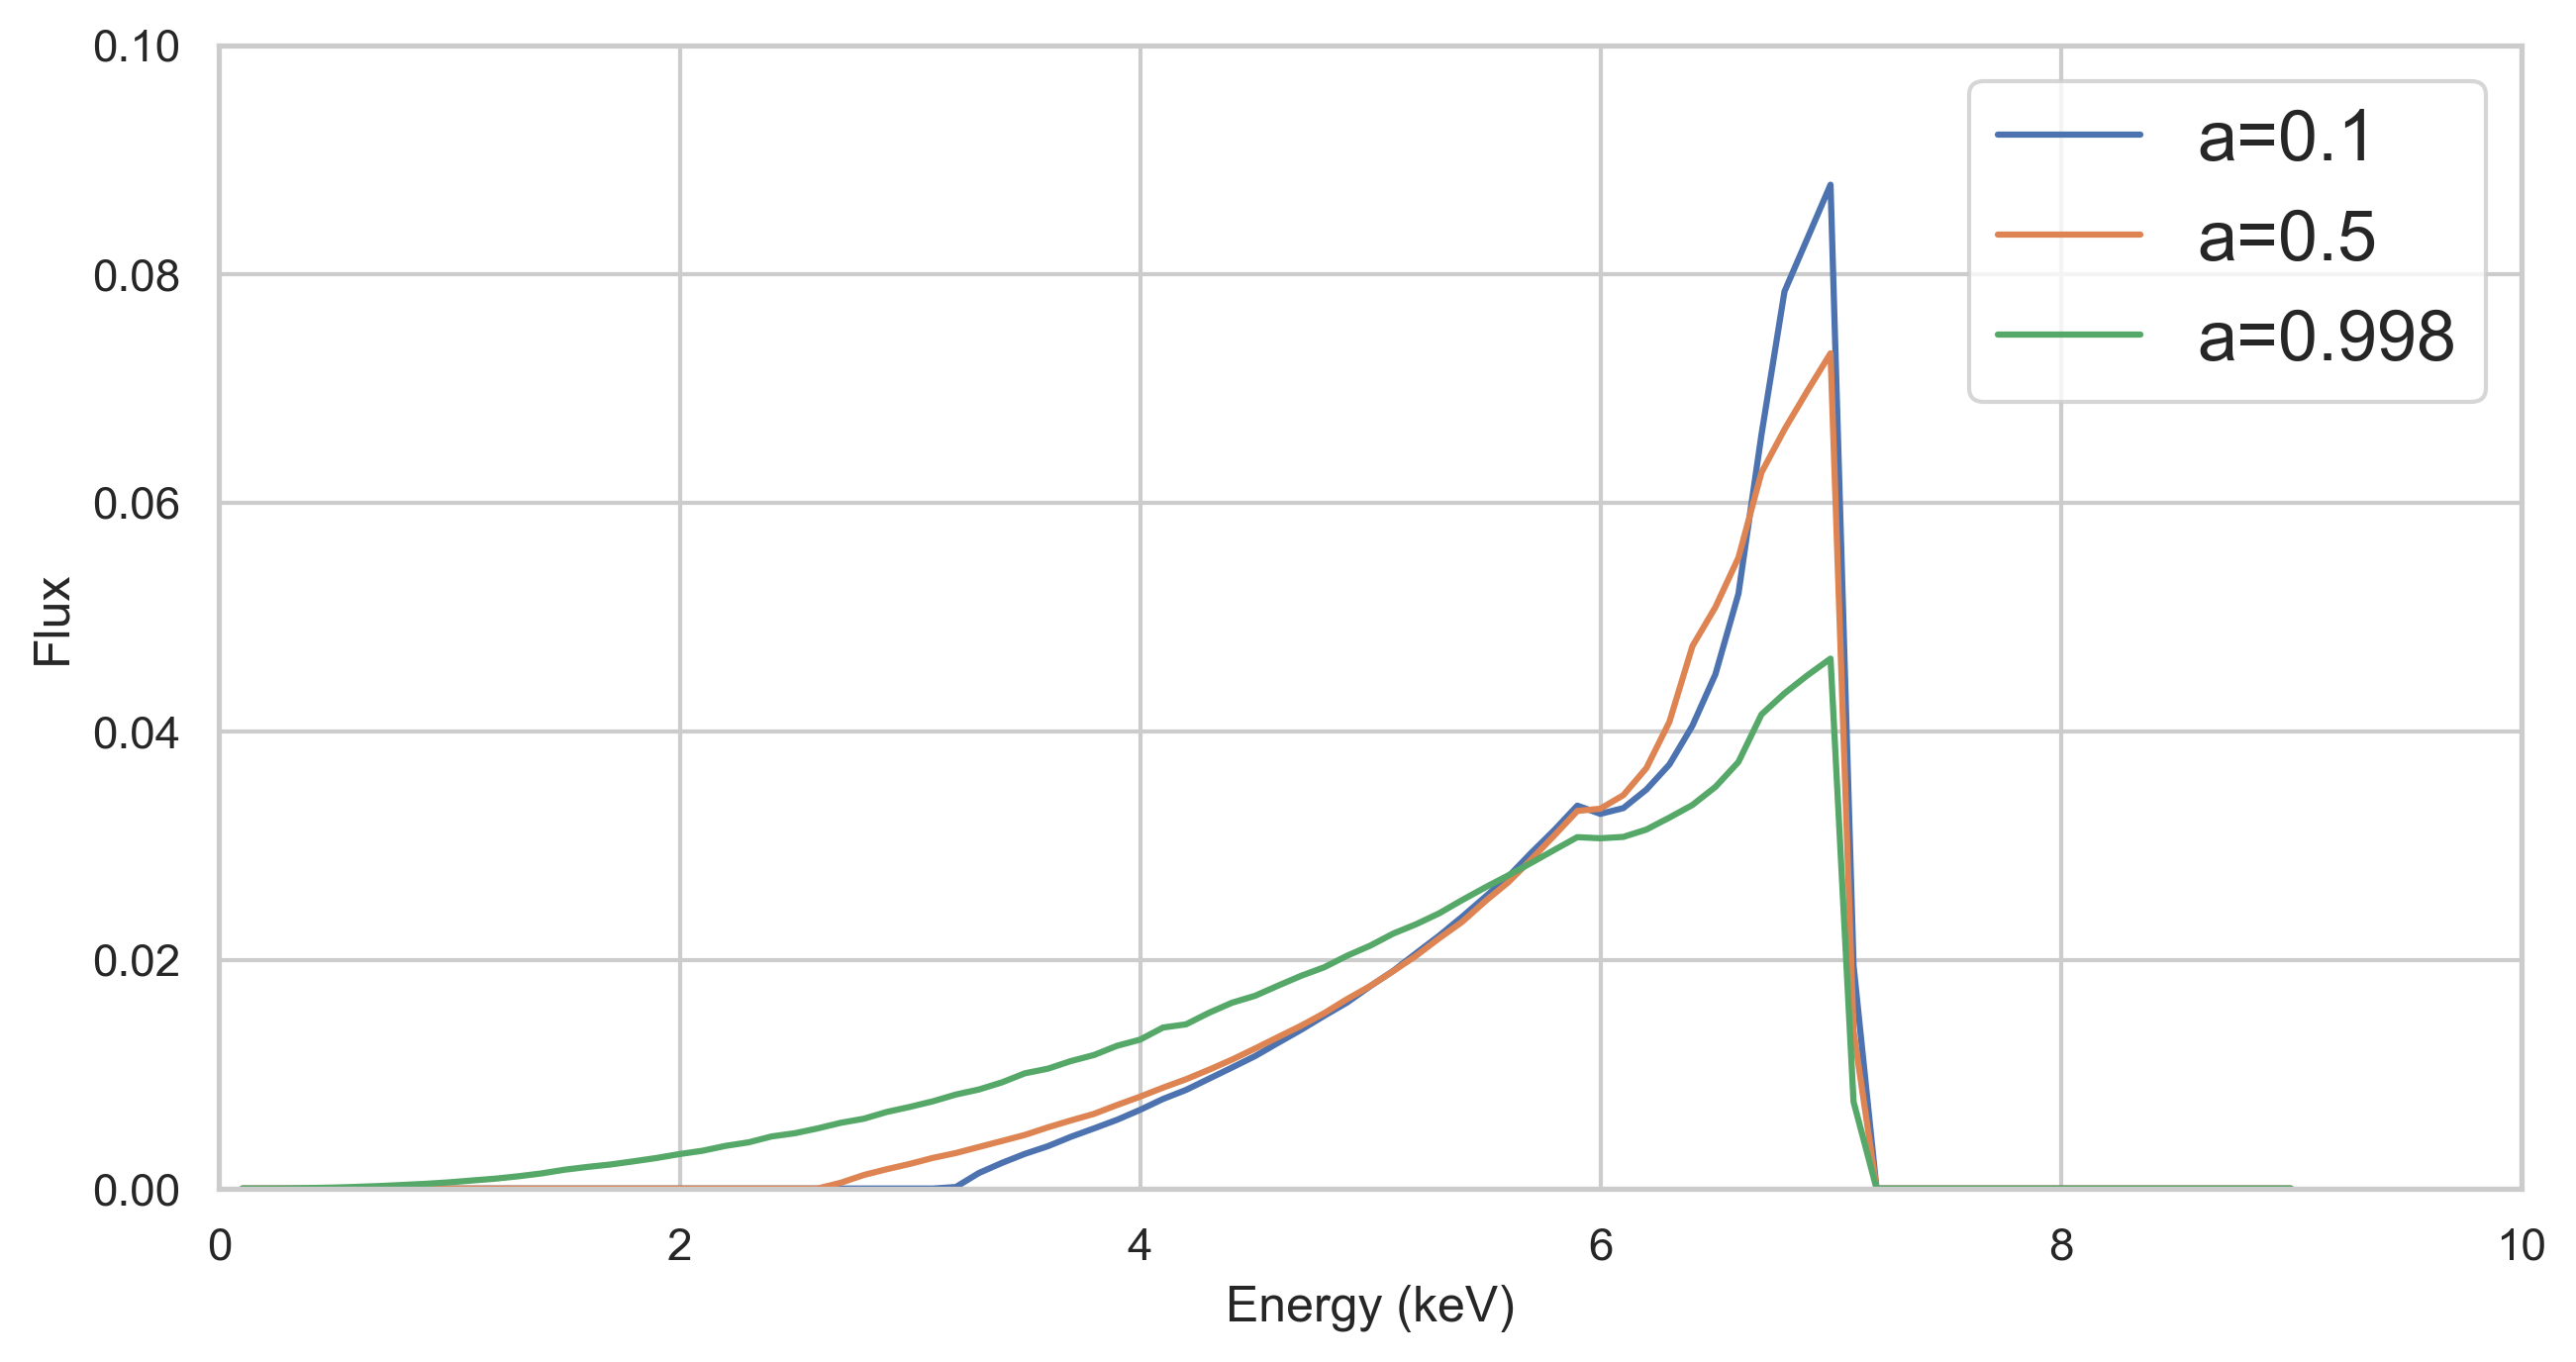
\includegraphics[width=0.90\textwidth]{asset/spectrum.png}
\end{frame}


\section{Concluding Remarks}


\begin{frame}{Concluding Remarks}
    \Large
    What have we learnt?
\end{frame}


\begin{frame}{Concluding Remarks}
    \Large
    Similar mathematical ideas arise from distinct physical principles.
\end{frame}


\begin{frame}{Concluding Remarks}
    \Large
    In tackling the most difficult questions, human ingenuity prevails over computational brute force.
\end{frame}


\begin{frame}{}
    \begin{center}
        {\Huge Thank you!}
    \end{center}
\end{frame}


\begin{frame}{}
    \centering

    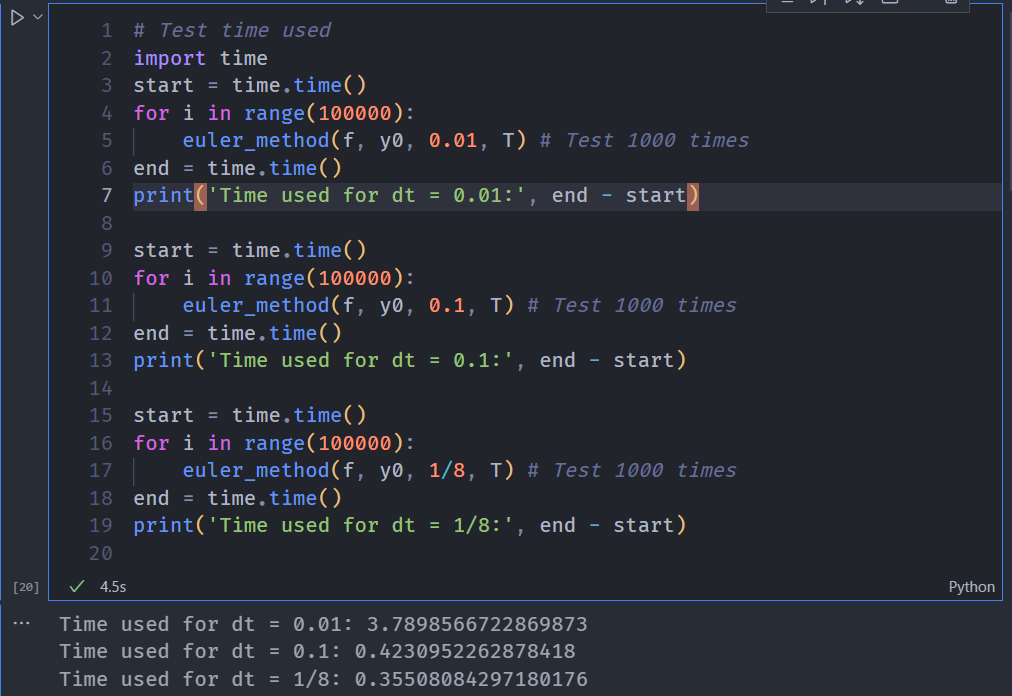
\includegraphics[width=\textwidth]{asset/speed_test.png}

    \footnotetext{Time comparison}
\end{frame}


\begin{frame}{}
    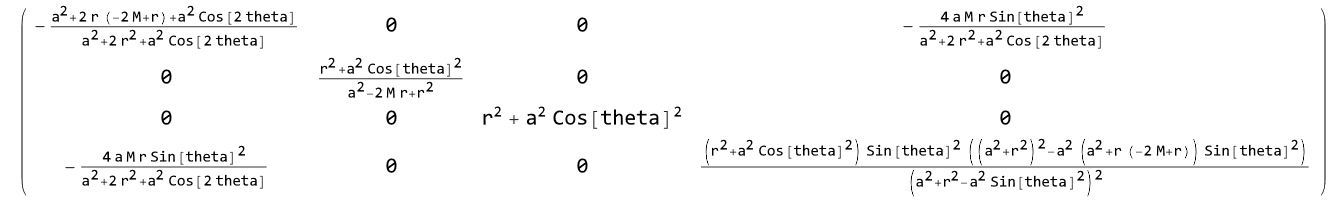
\includegraphics[width=\textwidth]{asset/kerr_metric.png}

    \footnotetext{Kerr metric}
\end{frame}


\begin{frame}{}
    \centering

    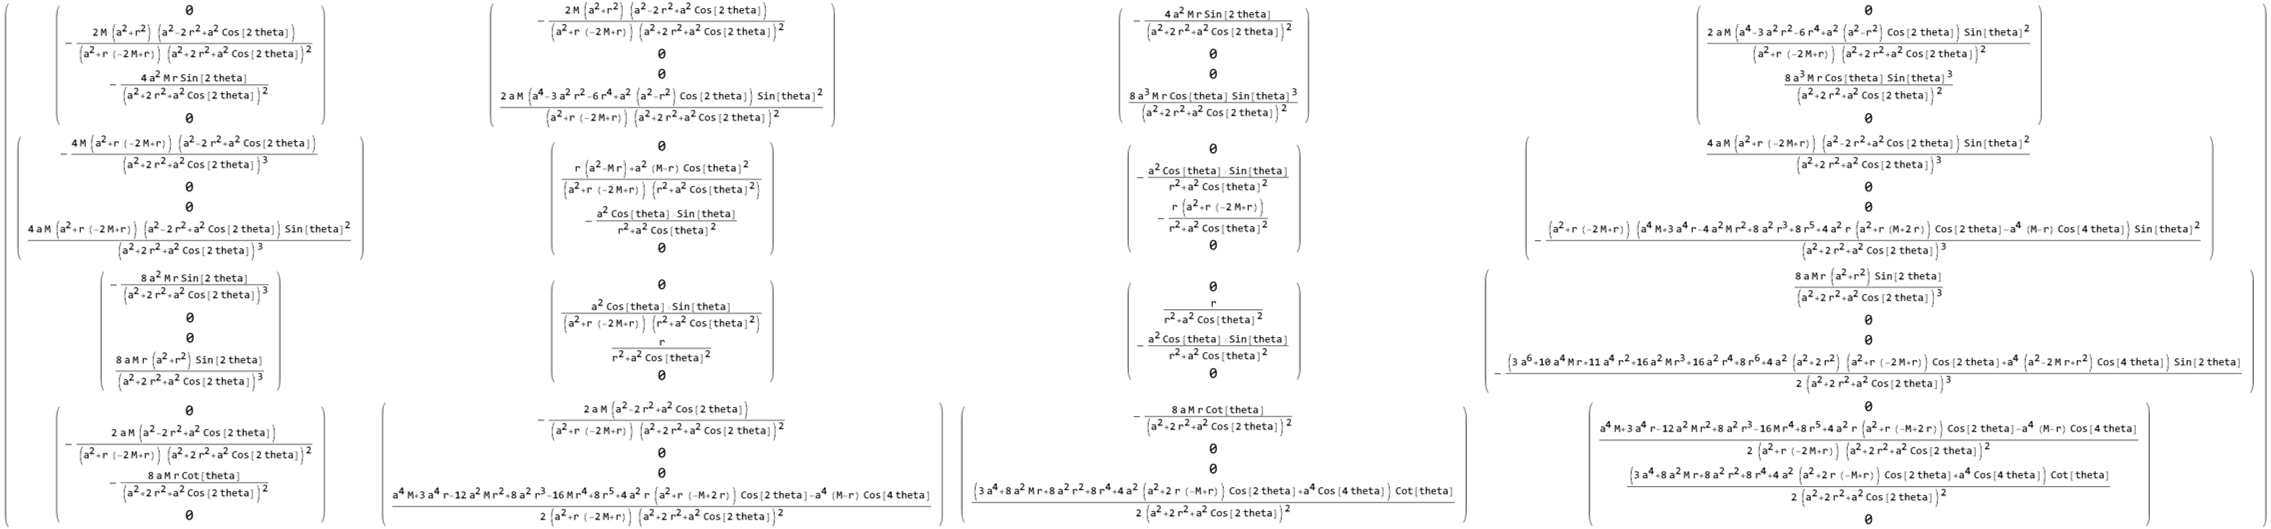
\includegraphics[width=\textwidth]{asset/christ.png}

    \footnotetext{Christoffel symbols of Kerr metric}
\end{frame}


\begin{frame}{}
    \centering

    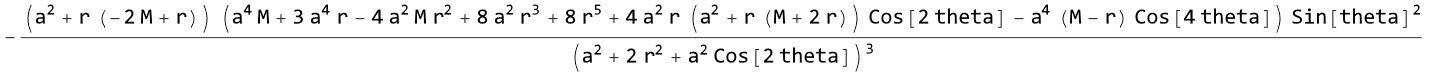
\includegraphics[width=\textwidth]{asset/christ_detail.png}

    \footnotetext{An element of the Christoffel symbols}
\end{frame}


\begin{frame}{}
    \centering

    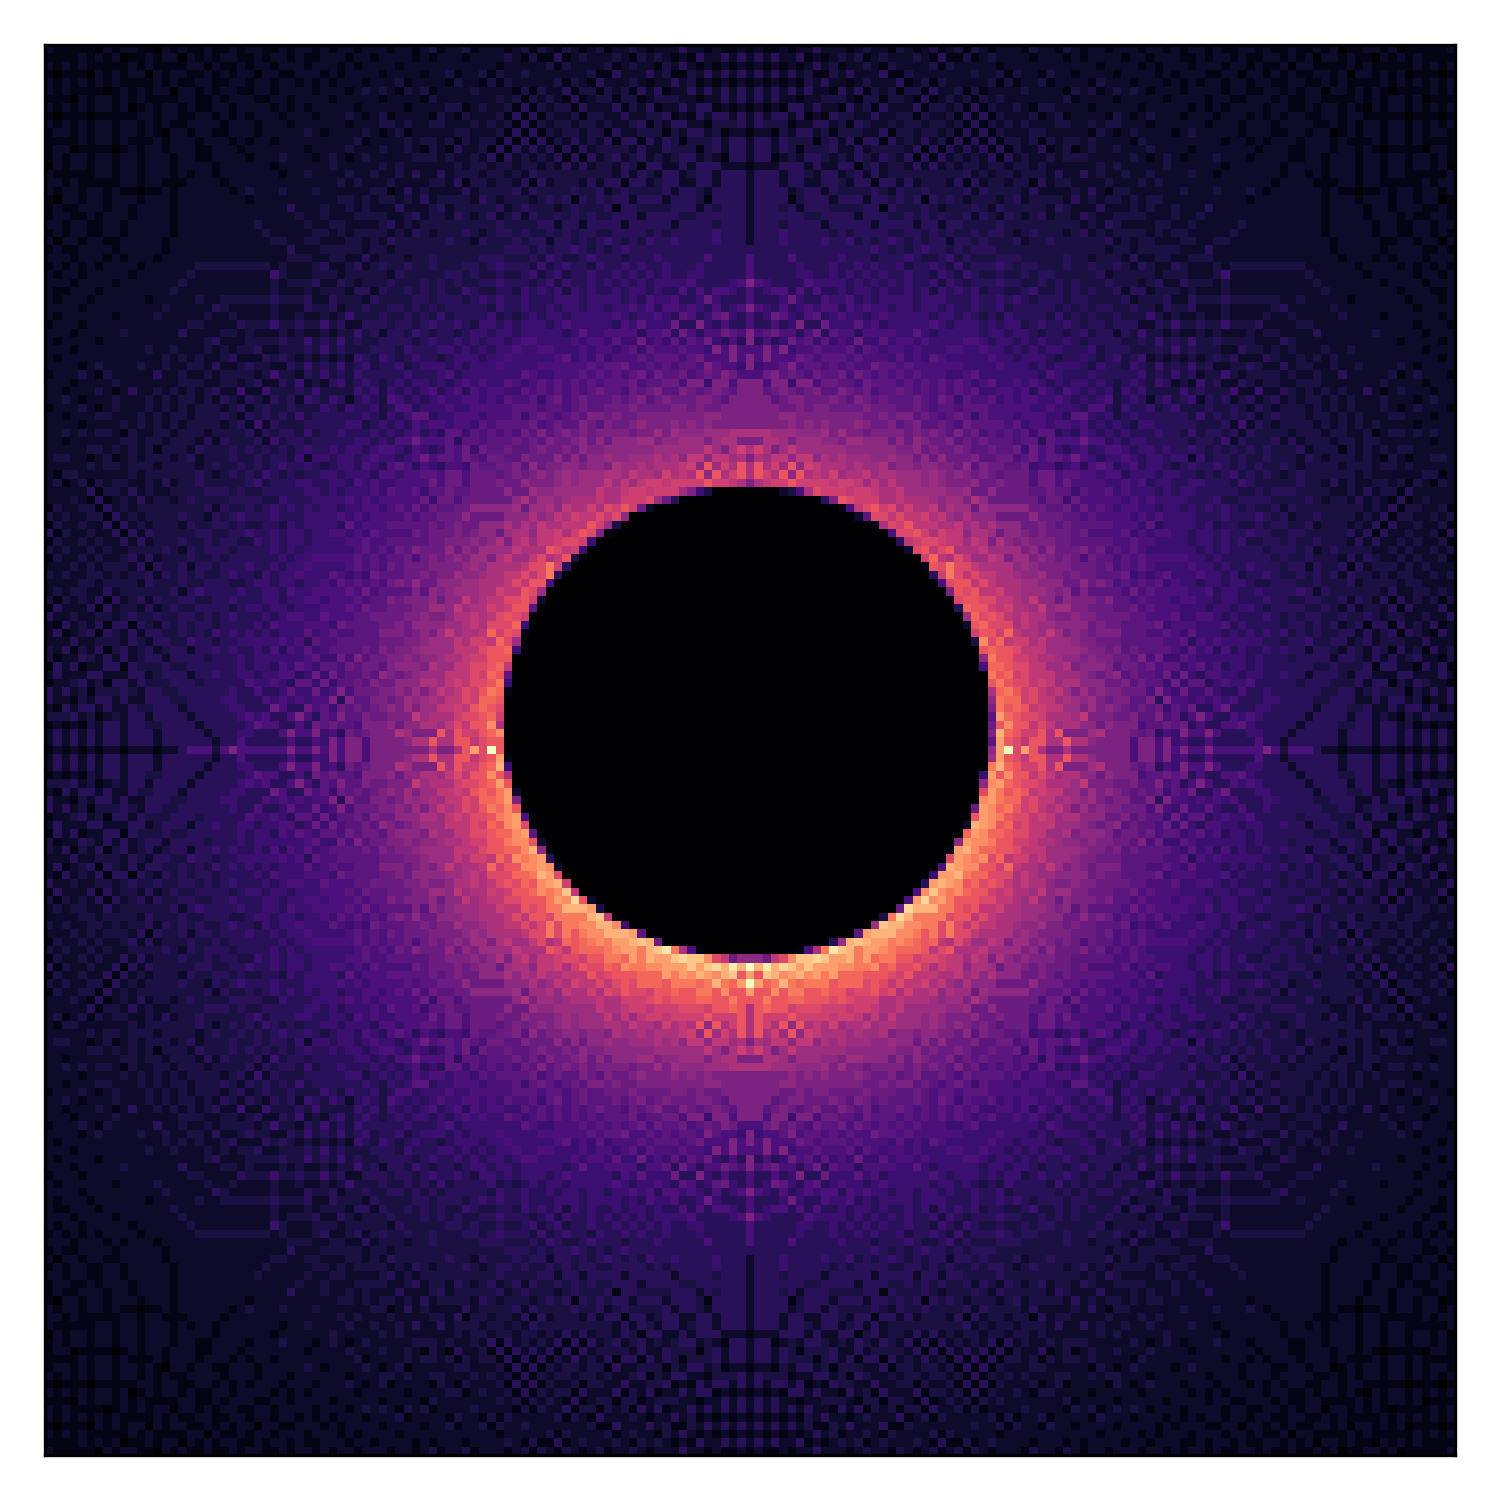
\includegraphics[width=0.8\textwidth]{asset/bh_0.5_20.png}

    \footnotetext{spin = 0.5, inclination = 20 deg}
\end{frame}


\begin{frame}{}
    \centering

    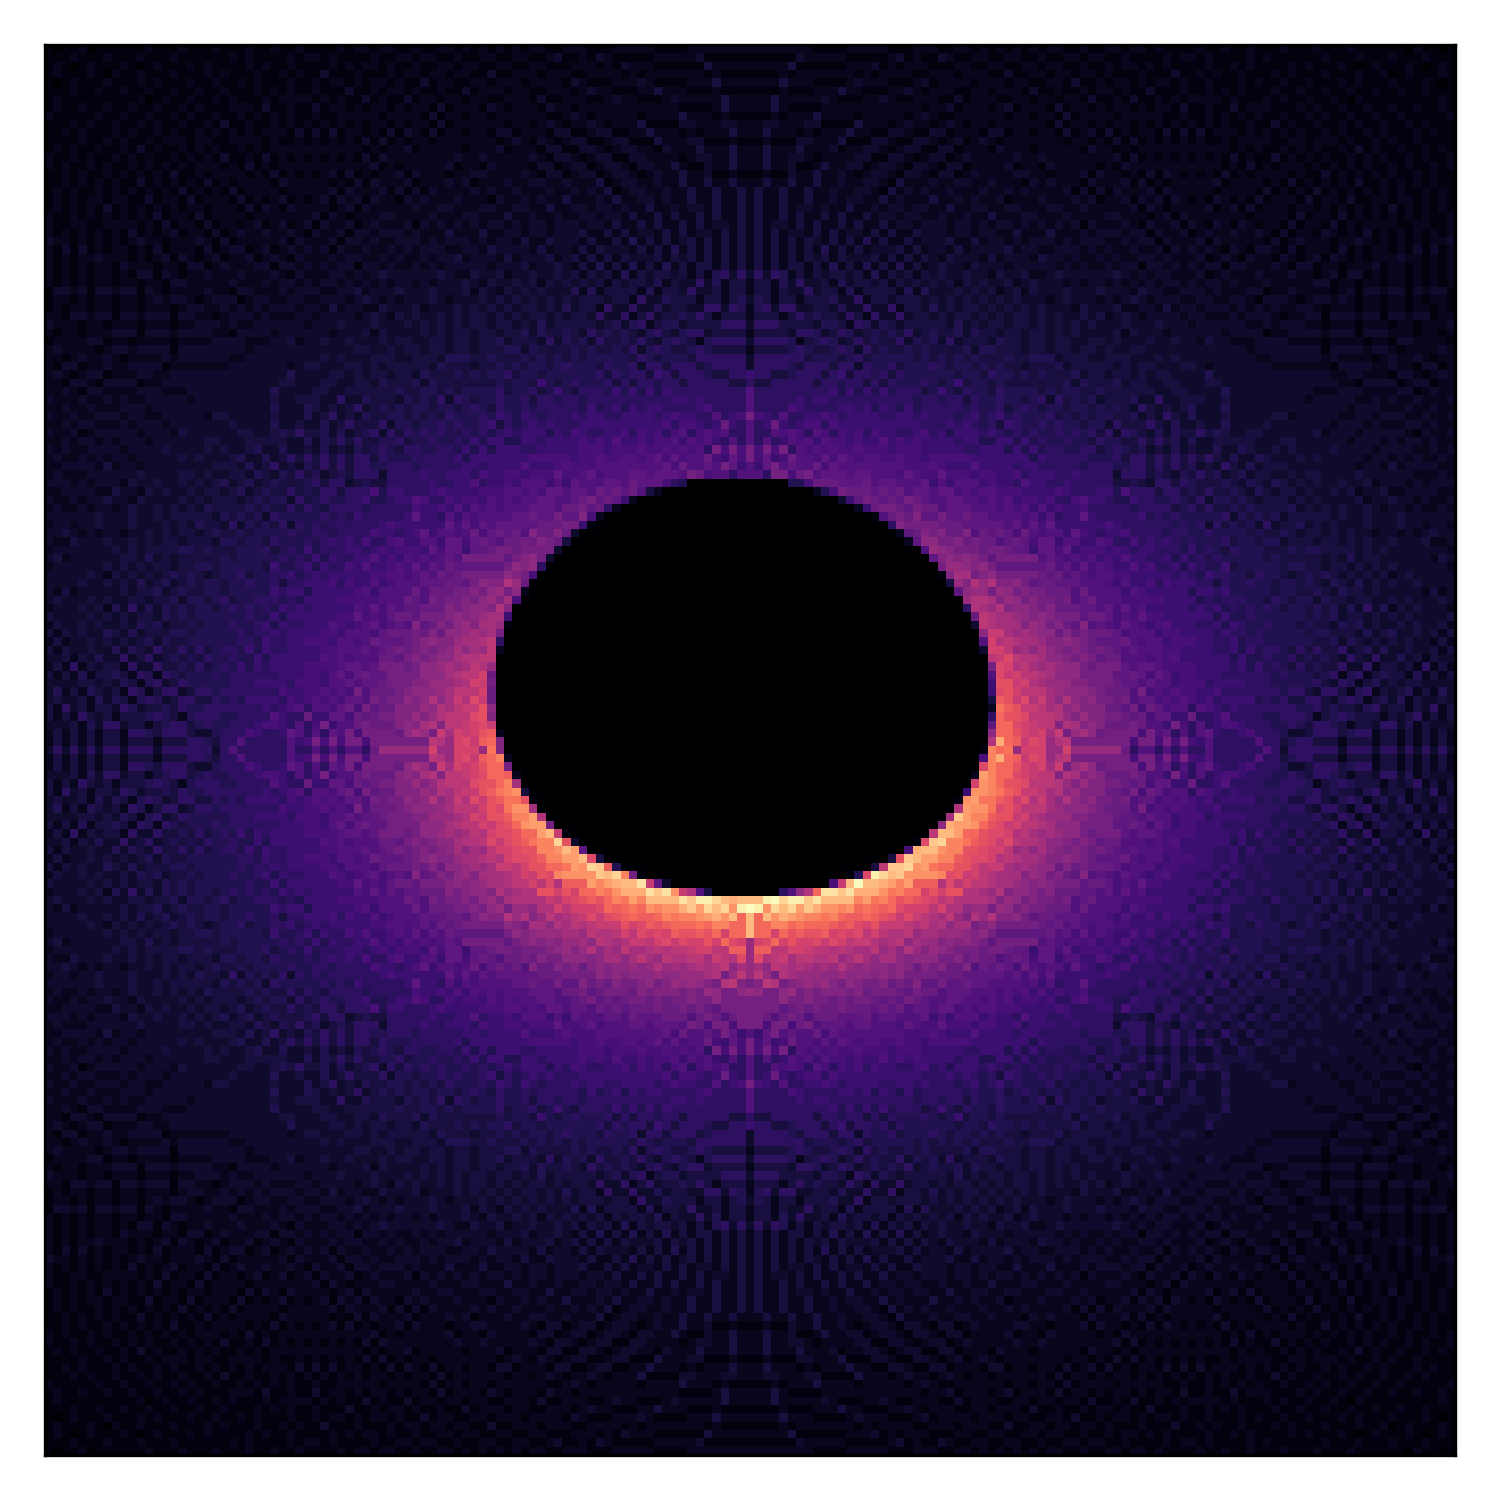
\includegraphics[width=0.8\textwidth]{asset/bh_0.5_45.png}

    \footnotetext{spin = 0.5, inclination = 45 deg}
\end{frame}


\begin{frame}{}
    \centering

    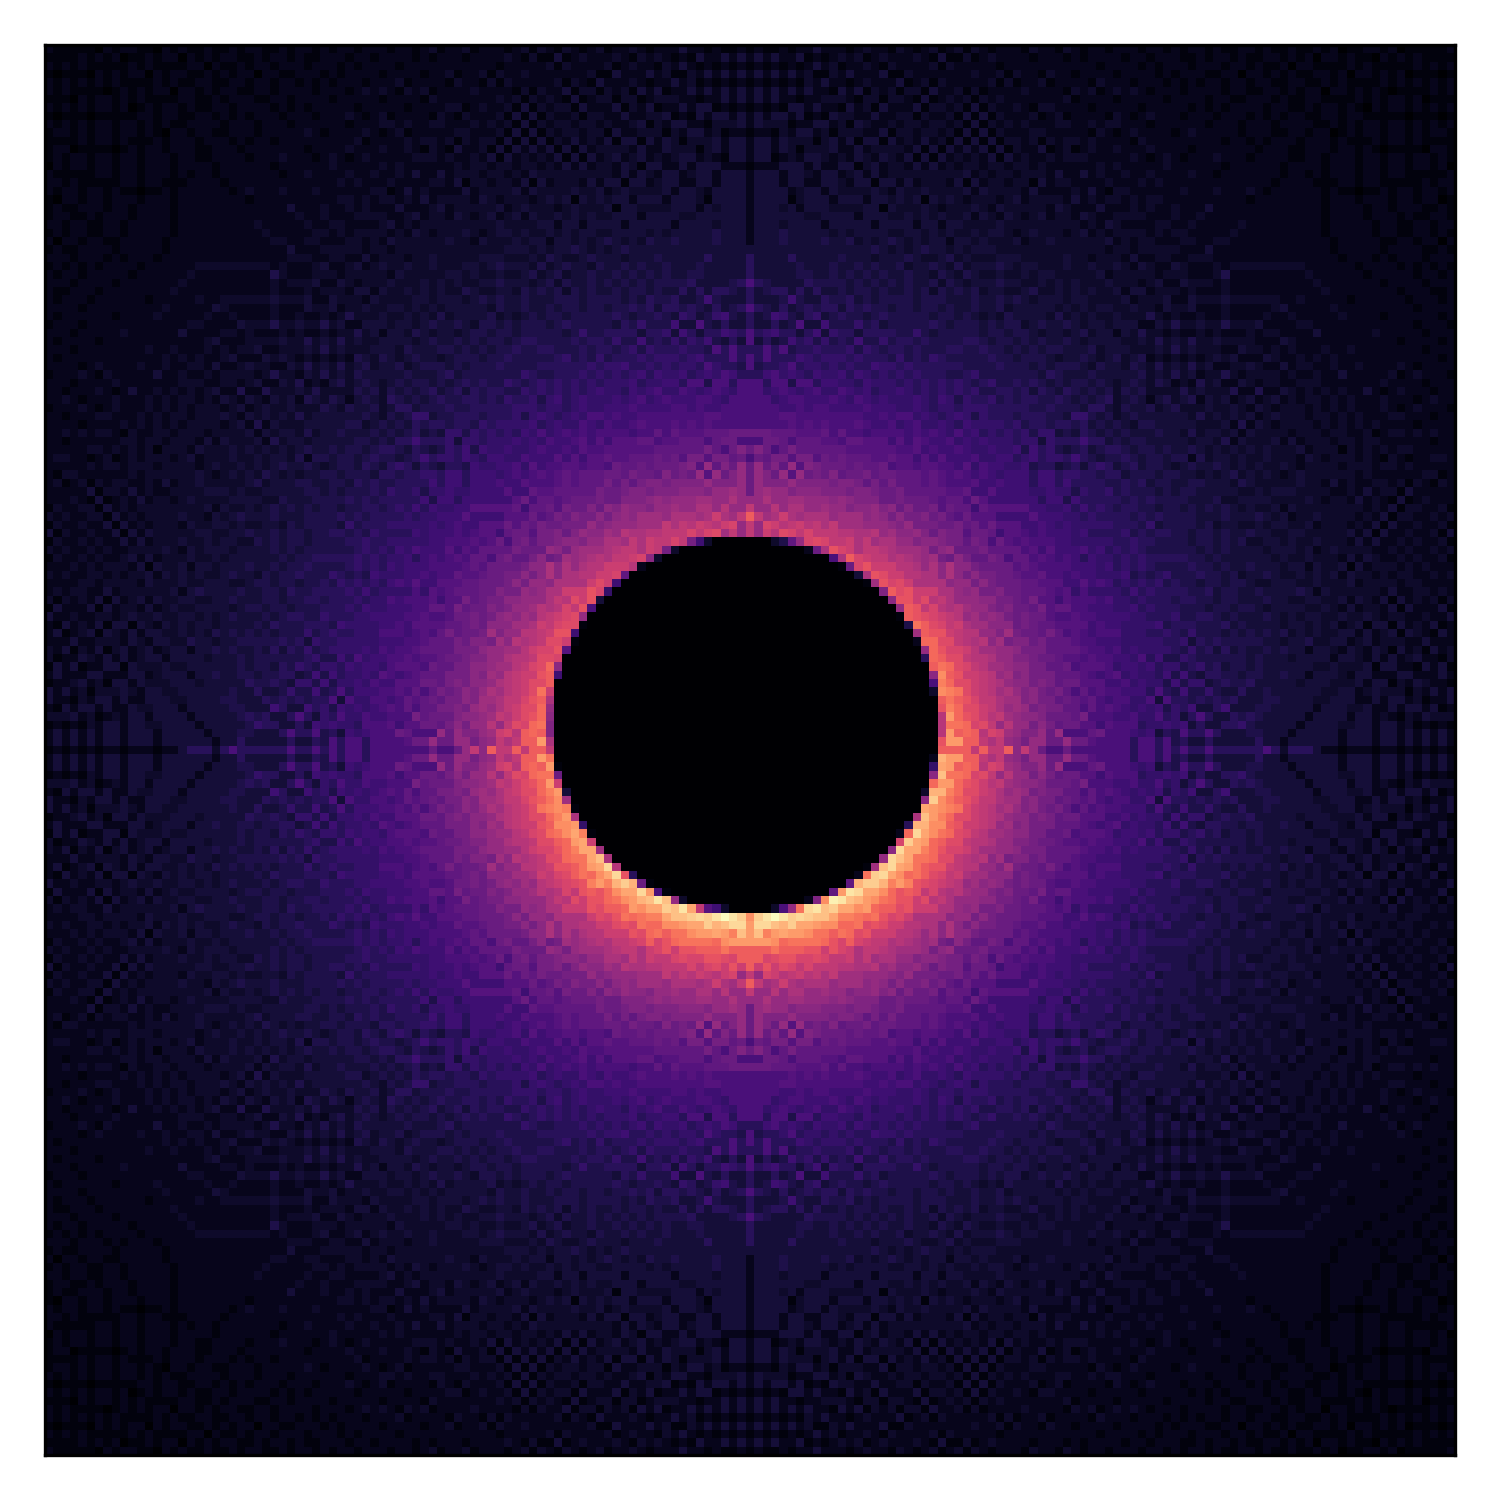
\includegraphics[width=0.8\textwidth]{asset/bh_0.75_20.png}

    \footnotetext{spin = 0.75, inclination = 20 deg}
\end{frame}


\begin{frame}{}
    \centering

    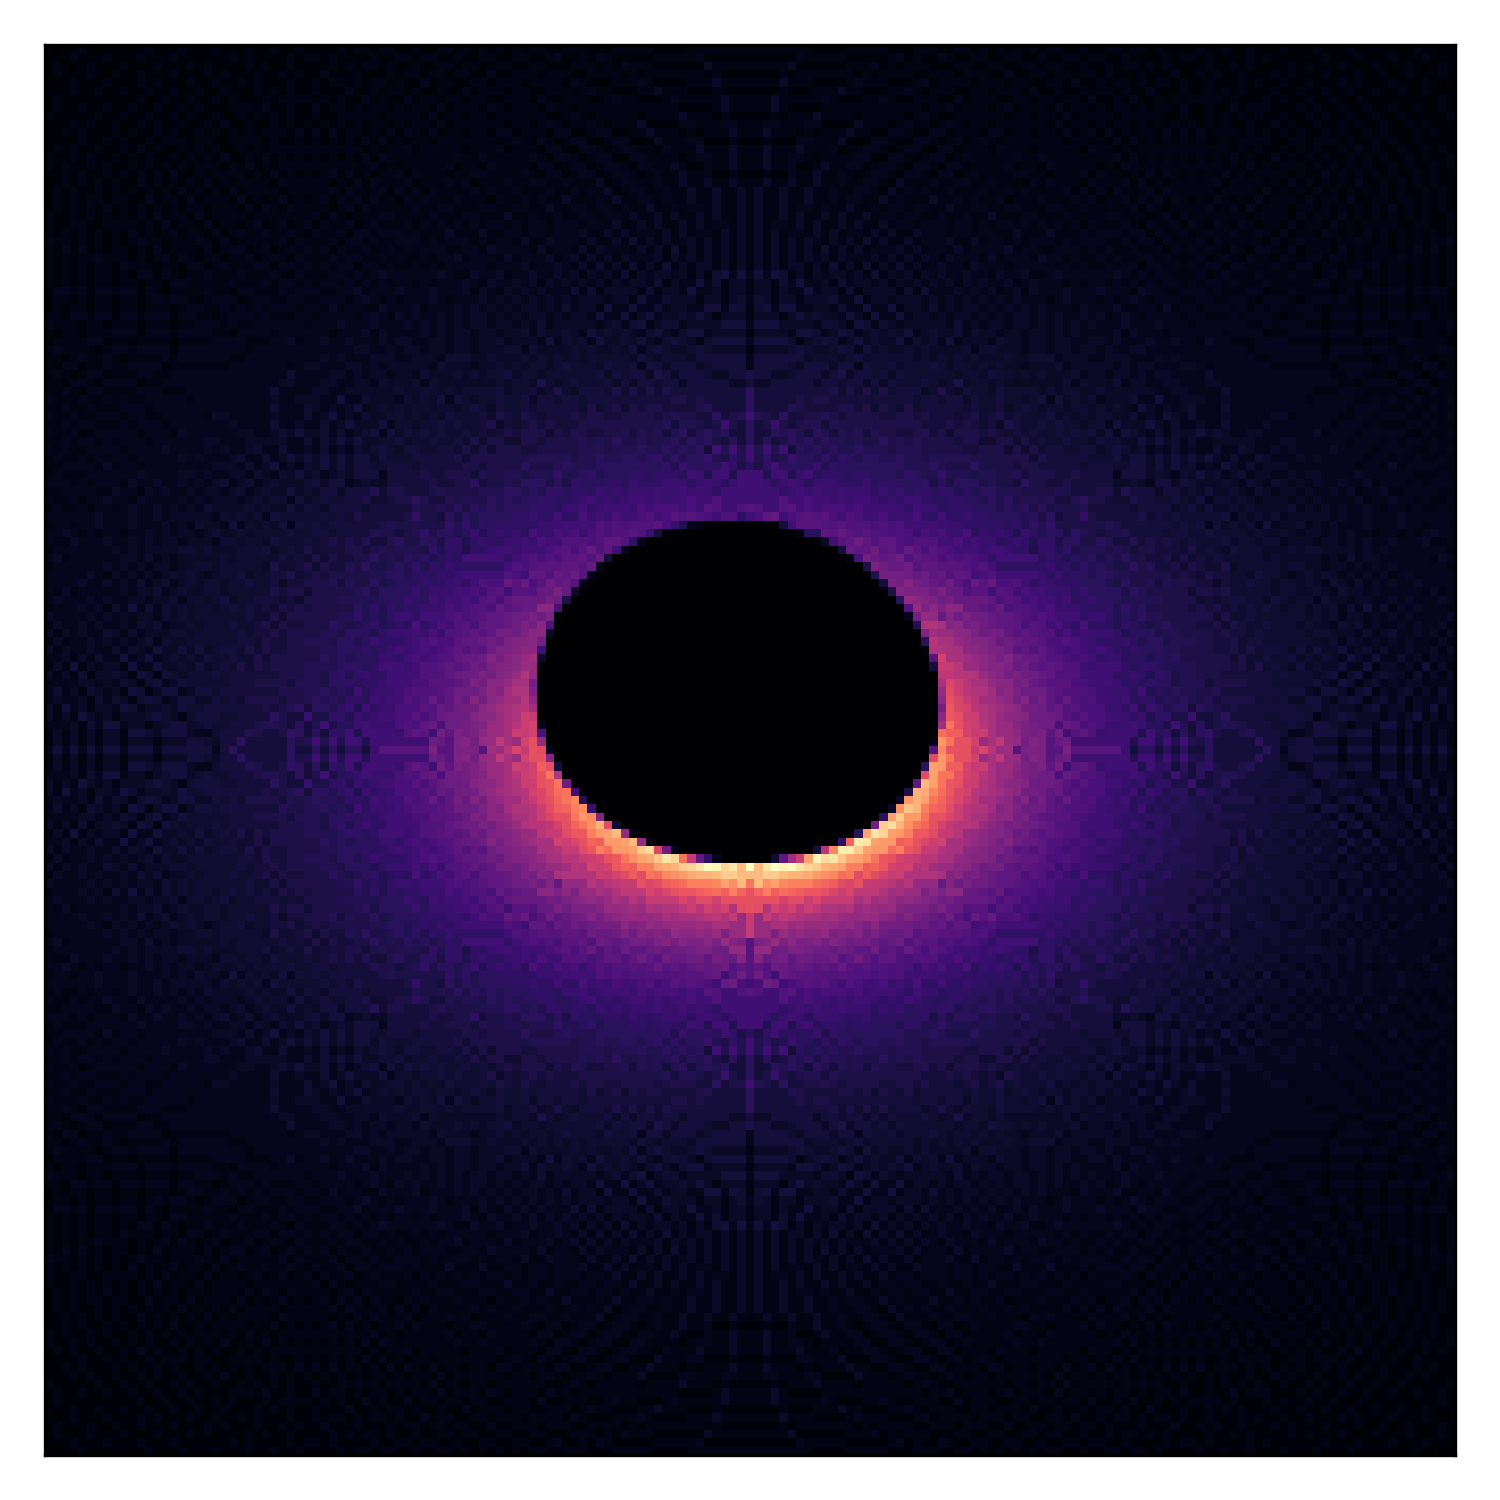
\includegraphics[width=0.8\textwidth]{asset/bh_0.75_45.png}

    \footnotetext{spin = 0.75, inclination = 45 deg}
\end{frame}


\begin{frame}{}
    \centering

    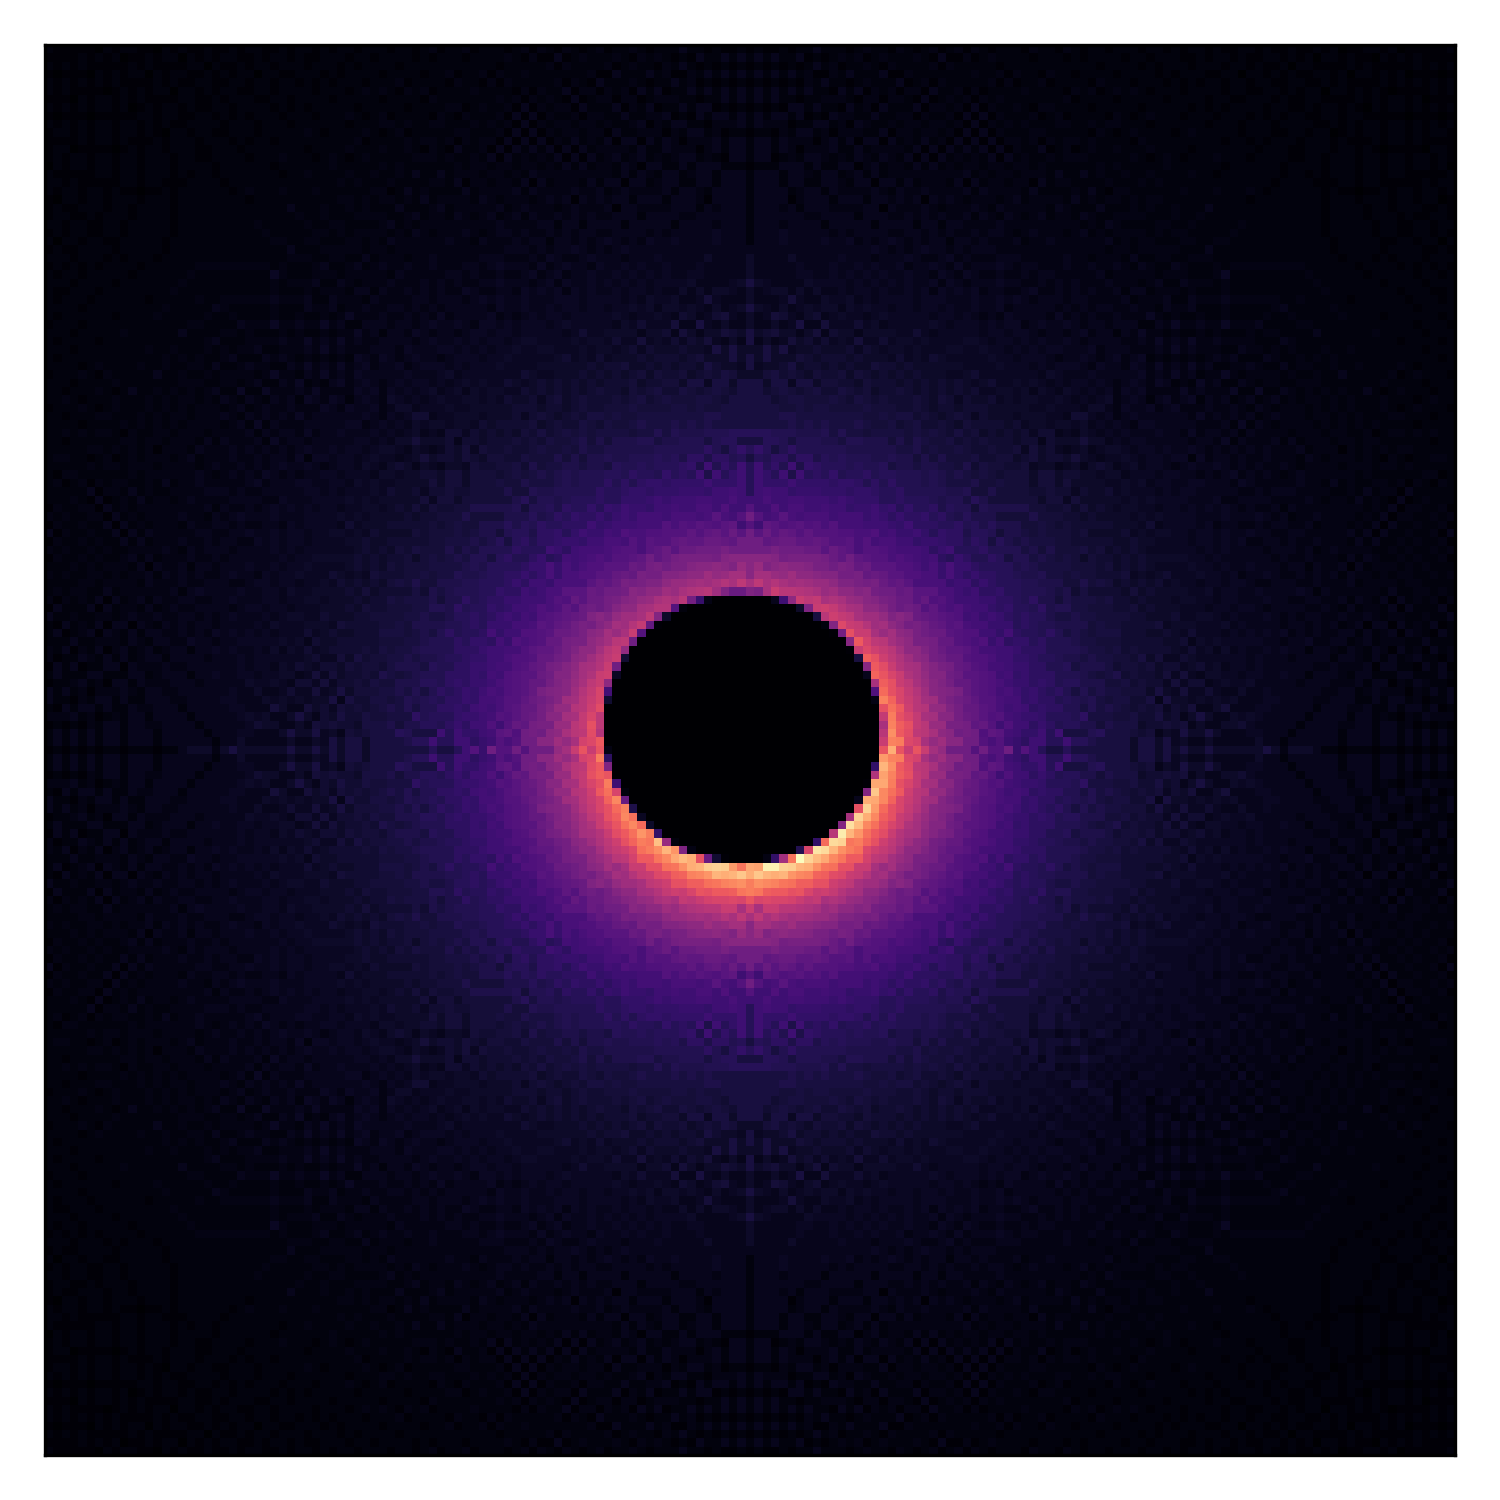
\includegraphics[width=0.8\textwidth]{asset/bh_0.95_20.png}

    \footnotetext{spin = 0.95, inclination = 20 deg}
\end{frame}


\begin{frame}{}
    \centering

    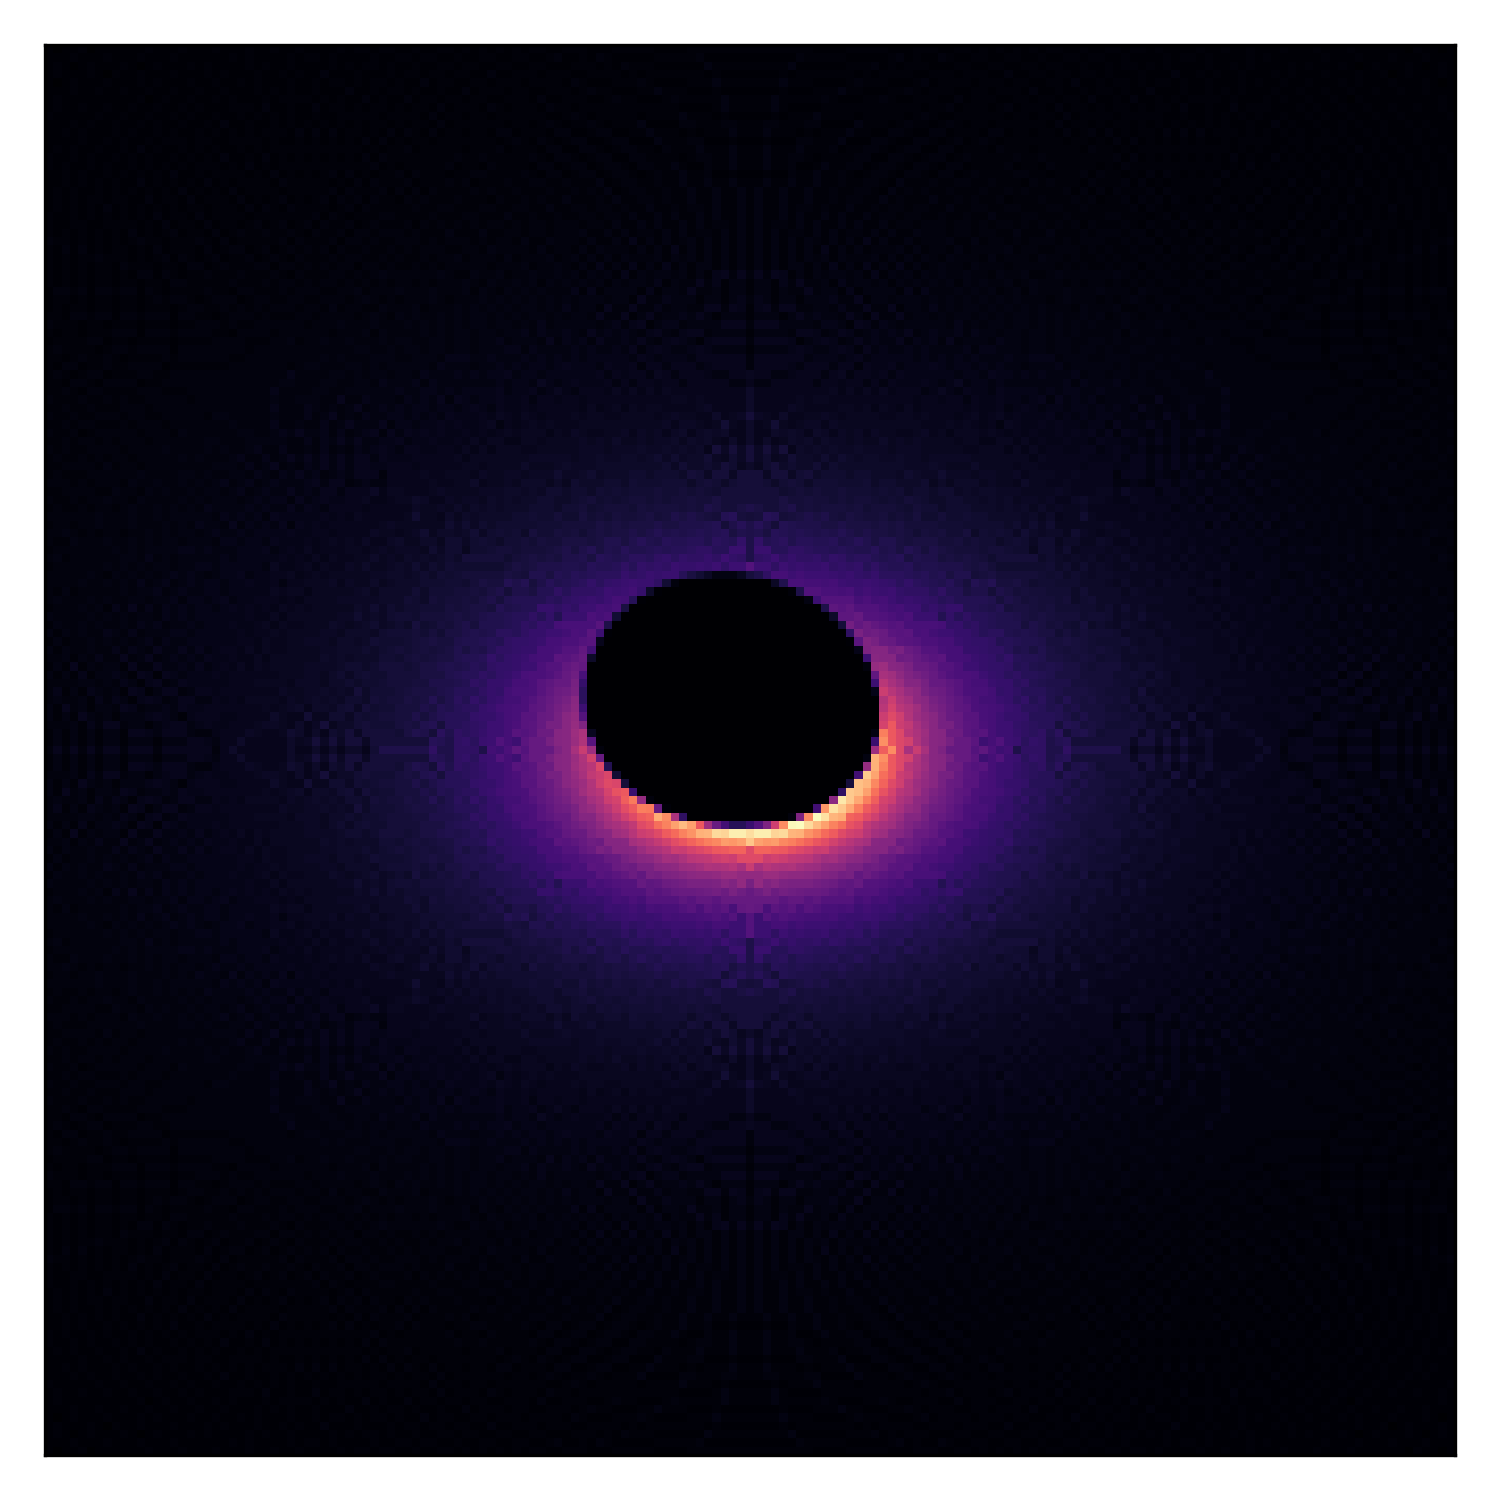
\includegraphics[width=0.8\textwidth]{asset/bh_0.95_45.png}

    \footnotetext{spin = 0.95, inclination = 45 deg}
\end{frame}


\end{document}